% CHAPTER 3

\chapter{BACKGROUND}
\label{chp:background}
#TODO write

\section{Event Log}
\label{sec:event-log}
Event logs are the main inputs to any process mining methodology including this thesis study and they include information related to real life activities. Event logs which are the outputs of the software systems like Enterprise Resource Planning (ERP) or Business Process Management (BPM) have common properties that are also assumed in the literature as the properties of event logs. General structure of event logs includes multiple layers as diagrammed in Figure~\ref{fig:event-log-structure}. Processes have cases which are simply single process instances. Within each case, there are events that are generally represents a sequence of activities performed. Each event is enhanced with the attributes such as timestamps, resource assignments and other contextual data. A fragment of this structure is presented in Table~\ref{table:event-log-loan} for the Loan Application Process, which shows the footprints of a financial organization that provides consumer credits \cite{buijs2013improving}. In the table, each line represents an event with its attributes which are collected under cases to form a complete event log. 

#TODO event log referansı koy

\begin{figure}
  \centering
  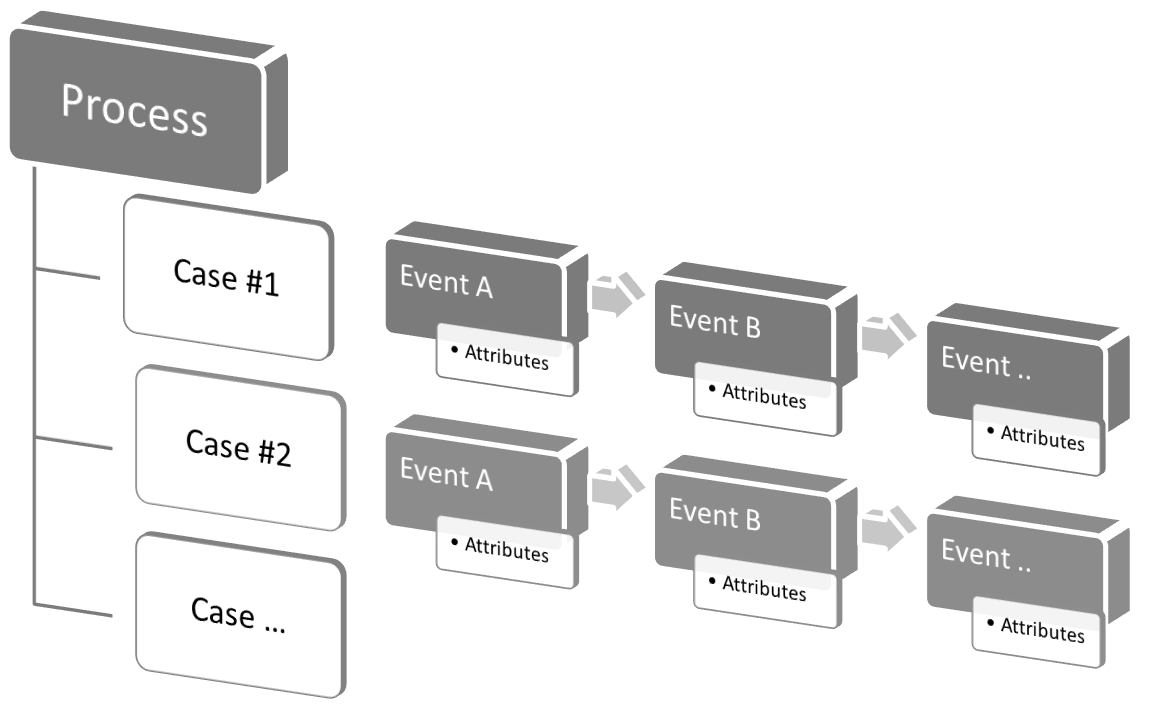
\includegraphics[width=\textwidth]{3_background/event_log_structure}
  \caption{Structure of Event Logs}
  \label{fig:event-log-structure}
\end{figure}

\begin{table}[h]
\centering
\caption{Fragment of event log from Loan Application Process (Variation #1)}
\label{table:event-log-loan}
\begin{tabular}{@{}llccc@{}}
\toprule
\multicolumn{5}{c}{\textbf{Event Log}}                                                                  \\ \midrule
                        &                         & \multicolumn{3}{c}{\textbf{Attributes}}             \\ \midrule
                        & \textbf{Event}          & \textbf{Date} & \textbf{Time} & \textbf{Transition} \\ \midrule
\textbf{Case \#1}       & Register Application    & 16.04.2013    & 14:37:27      & Complete            \\ \midrule
                        & Check Credit            & 16.04.2013    & 14:41:19      & Complete            \\ \midrule
                        & Check System            & 16.04.2013    & 14:47:35      & Complete            \\ \midrule
                        & Calculate Capacity      & 16.04.2013    & 14:50:21      & Complete            \\ \midrule
                        & Accept                  & 16.04.2013    & 14:53:22      & Complete            \\ \midrule
                        & Send decision e-mail    & 16.04.2013    & 14:55:11      & Complete            \\ \midrule
\textbf{Case \#2}       & Register Application    & 16.04.2013    & 16:28:19      & Complete            \\ \midrule
                        & Check Credit            & 16.04.2013    & 16:36:22      & Complete            \\ \midrule
                        & Check System            & 16.04.2013    & 16:43:10      & Complete            \\ \midrule
                        & Calculate Capacity      & 16.04.2013    & 16:52:40      & Complete            \\ \midrule
                        & Reject                  & 16.04.2013    & 16:53:53      & Complete            \\ \midrule
                        & Send decision e-mail    & 16.04.2013    & 17:01:32      & Complete            \\ \midrule
\multicolumn{1}{c}{...} & \multicolumn{1}{c}{...} & ...           & ...           & ...                 \\ \bottomrule
\end{tabular}
\end{table}

Event log structure and related notions are formalized in \cite{van2011process} as following:

\theoremstyle{definition}
\begin{definition}{}
(Event and Event Attributes) Let \textit{E} be the universe of events which include all possible event identifiers. In this universe any event \textit{e} $\in$ \textit{E}. Events are enhanced with contextual information, namely attributes. For any event \textit{e} $\in$ \textit{E} and attribute \textit{A}, $\#_\textit{A}(\textit{e})$ is the value of the attribute \textit{A} for event \textit{e}. Possible attributes for events include timestamps, people and resource assignments, transaction types and other contextual data.
\end{definition}

\theoremstyle{definition}
\begin{definition}{}
(Case and Case Attributes) Let \textit{C} be the universe of cases which include all possible case identifiers. In this universe any case \textit{c} $\in$ \textit{C}. Like events, cases are also enhanced with contextual information, namely attributes. For any case \textit{c} $\in$ \textit{C} and attribute \textit{A}, $\#_\textit{A}(\textit{c})$ is the value of the attribute \textit{A} for case \textit{c}. Each case has at least one attribute which is trace.
\end{definition}

\theoremstyle{definition}
\begin{definition}{}
(Trace) Trace is a sequence of event \textit{t} $\in$ $\textit{E}^*$ such that each event is restricted to occur only once.
\end{definition}

\theoremstyle{definition}
\begin{definition}{}
(Event Log) Event log is set of cases \textit{L} $\subseteq$ \textit{C} such that each event occurs at most one in the event log.
\end{definition}

In this study, event logs from different organizations are exploited, thus organization related attributes are used for cases. Within these event logs, traces of cases for each organizational is used to discover underlying process models. In addition, timestamp and resource related attributes of events are used to collect performance related data for further analysis.

\section{Process Modeling}
\label{sec:process-modeling}
Process modeling is the foundation of process management applications and main tools of people in this profession. Although process modeling can be defined with informal process workflows to document procedures, there are a number of formalized notations which are more suitable to cross-applicability and mathematical analysis. In the control-flow view of process modeling, a process model is aimed to give decisions on which activities to take place with their orders. In this study, control-flow of process models are used to find mismatch patterns between different organizations that execute the same activities. Considering the scope of this  thesis, only Petri nets, Workflow Nets and Business Process Modeling Notation(BPMN) will be presented since they are related. 

\subsection{Petri Nets}
\label{sec:petri-nets}
Petri net is a mathematical modeling language that is aimed to describe concurrent systems. Graphical notation of Petri nets seems intuitive and simple; however, it is powerful in terms of being executable and applicability of analysis techniques \cite{vanderAalst:2011:MBP:2000715}. Petri nets are directed bipartite graphs where nodes \textit{represent} transitions and \textit{places} represent conditions. Structure represented by Petri nets is static and the state of the net is described by placint \textit{tokens}, namely the process of \textit{marking}. Formalization of Petri nets are explained in \cite{reisig1998lectures} as following:

\theoremstyle{definition}
\begin{definition}{}
(Petri Nets) A \textit{Petri net} is a triplet $N = (P, T, F)$ where $P$ is finite set of \textit{places}, $T$ is finite set of \textit{transitions} and $F$ is set of \textit{flow relations} where:
\begin{enumerate}
  \item (Seperation) $P \cap T = \varnothing$
  \item (Flow relation) $F \subseteq (P \times T) \cup (T \times P)$
\end{enumerate}
\end{definition}


\subsection{Workflow Nets}
\label{sec:workflow-nets}
Process models in the real life have additional properties to be executable and they are defined in the Workflow net formalization, which is simply a subset of Petri nets. These additional properties can be formalized as following \cite{van2013discovering}:
\theoremstyle{definition}
\begin{definition}{}
(Workflow Nets) Let $N = (P, T, F)$ be a Petri net and $t$ is a new identifier not in $P \cup T$. $N$ is a workflow net (WF-net) if and only if:
\begin{enumerate}
  \item (Start Node) $P$ contains a \textit{source place i} where no token can be fired to.
  \item (End Node) $P$ contains a \textit{sink place o} where no token can be fired from.
  \item (Connectedness) $\bar{N} = (P, T \cup \{t\}, F \cup \{(o,t),(t, i)\})$ is strongly connected, in other words there is a directed path between any pair of nodes in $\bar{N}$.
\end{enumerate}
\end{definition}

In simple terms, a Workflow net is a Petri net with a source place to start the process starts and a sink place to end; furthermore, all nodes are on a path from source place to sink place \cite{van1998application}.  In order to illustrate this formalization, the Workflow net for the event log mentioned in Section~\ref{sec:event-log} is presented in Figure~\ref{fig:loan-petri-net}. In the figure, places are indicated by circles, transitions are indicated by rectangles, and flow relations are represented by arcs. 
\begin{figure}
  \centering
  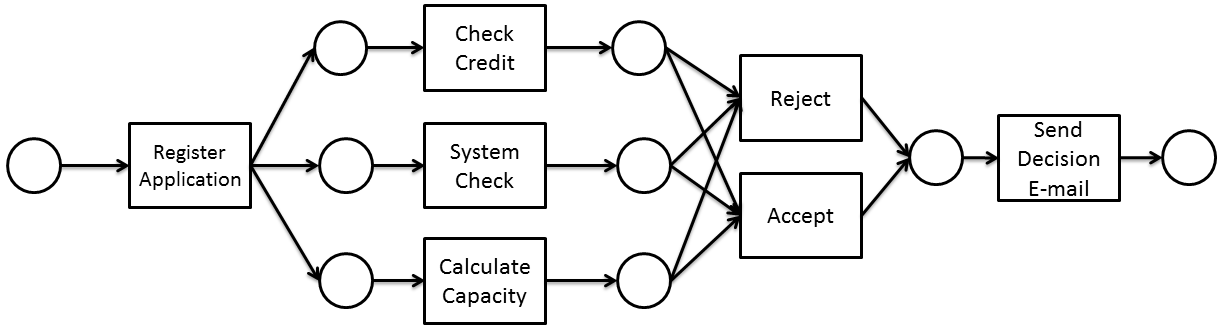
\includegraphics[width=\textwidth]{3_background/loan-petri-net}
  \caption{Workflow net of Loan Application Process (Variation #1)}
  \label{fig:loan-petri-net}
\end{figure}

Workflow nets are representative to real life processes; however, they can result with processes including deadlocks, livelocks and never-reached activities. In order to avoid process models from these problems, soundness definition is suggested in \cite{van1998application} and it is simplified as following with the context of this thesis:
\theoremstyle{definition}
\begin{definition}{}
(Soundness) Let $N$ be a Workflow net and it is sound if and only if:
\begin{enumerate}
  \item  (Safeness) Places cannot hold more than one tokens at the same time.
  \item  (Proper completion) Any marking of net can reach to sink place.
  \item  (Absence of dead tasks) Net does not contain any dead transitions.  
\end{enumerate}
\end{definition}

In this thesis, Workflow nets are used to discover and present underlying process models of different organizations. Considering the applicability of well-known process mining algorithms on Workflow nets and implementations in ProM Framework \cite{verbeek2010prom}, Workflow nets are used as the notation for discovery and analysis.

\subsection{Business Process Modeling Notation (BPMN)}
\label{sec:bpmn} 
Business Process Modeling Notation (BPMN) is one of the most popular and widely used modeling language implemented by many vendors. In addition to its popularity, this notation is standardized by the Object Management Group (OMG) since 2004. In this notation, atomic activities are named as \textit{tasks} and routing decision logic is implemented by \textit{gateways}. These gateways include split and join gateways with AND, OR and XOR logic operations. In addition, deferred choice pattern is implemented by \textit{event-based XOR gateway} in BPMN to handle race conditions between tasks that are running parallel \cite{van2003workflow}. Since the primary goal of BPMN is to provide a standardized notation that is easy to understand by business stakeholders, in this study resulting nets are converted to BPMN diagrams for visual analysis by the plugin implemented in ProM \cite{kalenkovaprocess}. BPMN diagram of the Workflow net from Figure~\ref{fig:loan-petri-net} is presented in Figure~\ref{fig:loan-bpmn}. As can be seen from the diagram, gateways help to understand the relations and dependencies of the tasks.

\begin{figure}
  \centering
  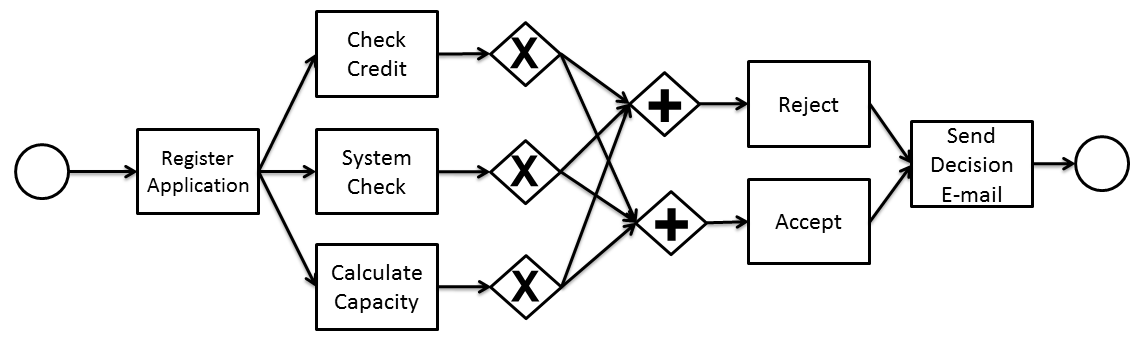
\includegraphics[width=\textwidth]{3_background/loan-bpmn}
  \caption{Process Model of Loan Application Process  (Variation #1) using BPMN}
  \label{fig:loan-bpmn}
\end{figure}


\section{Process Discovery}
\label{sec:process-discovery}
In process mining field, one of the most challenging task is to construct a process model based on the behavior in the event logs, namely process discovery. Many process discovery algorithms are proposed to address different challenges in process discovery and using different notations. However, in this thesis focus of the study is learning from the cross-organizational process mining rather than address all process discovery challenges. With this reasoning, Inductive Process Mining \cite{leemans2013discovering} is selected as appropriate since it is simple, highly applicable and configurable. In the literature, its derivatives which handles infrequent behaviors \cite{leemans2014discoveringinfrequent}; incomplete logs \cite{leemans2014discoveringincomplete}; and model optimization \cite{weidlich2012profiles} are also available.  

\textit{Inductive Miner (IM)}, which is proposed as an extensible framework in \cite{leemans2013discovering}, aims to discover block-structured process models that are sound and fitting to the behavior represented in event log. In addition, this approach focuses on creating rediscoverable models that is a key attribute in this study. Formalization of the key points in this study are as following:

\theoremstyle{definition}
\begin{definition}{}
(Block-structured Workflow Nets) Block-structured WF-nets are subset of WF-nets where the workflow can be divided recursively into  parts with single entry and exit points.  
\end{definition}

\theoremstyle{definition}
\begin{definition}{}
(Rediscoverability) Let a process is expressible by a model $M$ which is unknown priori. Given a log $L$ of $M$, $L$ is a subset of language used to describe model $M$. $M$ is isomorphic-rediscoverable from $L$ by mining algorithm $B$ if and only if $M \in B(L)$.
\end{definition}
 
Framework developed in the study \cite{leemans2013discovering} used a divide-and-conquer approach to discover subprocesses of sublogs obtained by splitting the event log. Main steps of the algorithm are listed as following:
\begin{enumerate}
  \item Activity Sets: Split the \textit{activities} in log to disjoint sets.
  \item Sublogs: Split the \textit{log} by using \textit{activity sets}.
  \item Recursive Mining: Mine sublogs with these steps until a sublog contains only single activity.
\end{enumerate}

In the study \cite{leemans2013discovering}, an algorithm based on this framework is presented that gurantees returning a sound and fitting process model in finite time. Therefore, this framework is selected as appropriate and its extension that can handle infrequent behavior which is used within this study to address challenges of different event logs. Frequent behavior is caused by the traces in the logs that might follow many different paths. In real life, these different paths are used infrequently; however, their effect in discovery is still significant. \textit{Inductive Miner Infrequent (IMi)} is proposed in \cite{leemans2014discoveringinfrequent} as an extension to \textit{Inductive Miner} to handle noise in the event logs. By filtering the infrequent behavior, it is aimed that \textit{IMi} succeeds with improved models discovered. After each recursive step of \texit{IM}, filtering is applied if the discovered model is a flower modek which represents infrequent behavior. Basic idea behind filtering is considering the trace and event frequency with a user-defined threshold between 0 to 1. Using this threshold, both log splittings and mining operations are done on a cleaner subset of logs. When the discovered models compared to \textit{IM}, \textit{IMi} results with lower fitness, higher precision and equal generalization.
In this thesis study, infrequent behavior capable implementation is used for experimenting the cross-organizational mining of process models with their implementation of ProM framework \cite{verbeek2010prom}.

\section{Replay Algorithm}
\label{sec:replay-algorithm}
#TODO write
% burayı 2.3.2'den performance ile enhance et

\section{Unsupervised Learning}
\label{sec:unsupervised-learning}
#TODO write

\subsection{K-means Clustering}
\label{sec:kmeans-clustering}
#TODO write

\section{Mismatch Patterns}
\label{sec:mismatch-patterns}
#TODO write